% !TeX root = ../main.tex

\chapter{THUR-20数据标准及校准技术规范}
\label{cha:chapter02}

\section{THUR-20设计目标}
\label{sec:design}
TODO

\section{THUR-20数据标准}
\label{sec:standard}

  THUR-20是一个基于UR5机械臂的的标准化抓取数据集,在采集过程中,它的主要设备
  及传感器组成有:

  \begin{itemize}
    \item 机械部分,UR5机械臂,Robotiq-2f-85夹爪;
    \item 传感器部分,包括视觉传感器以及触觉传感器;
    \item 逻辑控制部分,由一台配有i9 cpu、GeForce2080的笔记本组成;
  \end{itemize}

  符合规范的THUR-20数据应包含经过时间校准的机械臂关节角度序列,夹爪张角序列,
  俯视、斜视以及固定在夹爪手腕上的摄像头图片帧序列,这三个视角的图片序列应当
  全部为RGB-D图像,下面分段详述每个数据形式的具体要求和组织方式。

  数据组织方式:为了使THUR-20数据集标准具有泛化性且新手友好,我们使用一个顶端
  yaml文件维护每种数据流的种类、名字、及是否存在。若某个数据流(例如顶视RGB-D
  数据)在当前数据序列中是存在的,则数据录入者应当在顶层的yaml文件中注册本数据
  流,声明它的名字及数据种类。顶层yaml文件还有一个重要用途,是表明当前任务序列
  对应的任务种类及任务细分类别,e.g. short-task,pick-up。一个典型顶层yaml文件
  应当如下所示:

  BLABLABLA,TODO:贴一个带高亮的yaml文件上来,我还没有写。

  UR5机械臂的关节序列:机械臂的关节角度序列是本数据集的基础所在。本数据集中,
  UR5机械臂的数据帧包含5个部分,分别为:header, name, position, velocity, effort。
  header中存储了当前帧数据对应的时间戳,name为机械臂对应的关节的名字,为字符串
  向量,其后的三个向量中的数据顺序都应当对应name中的关节顺序。position为机械臂
  每个关节的转角,单位为rad;velocity为机械臂每个关节的角速度,单位为rad/s;
  effort为每个关节上检测到的扭矩,单位为Nm。在position,velocity,effort这
  三个数据位中,position是必须量,即若当前帧中不含position向量或者向量长度与
  name中的关节数目不符,则当前帧被判定为非法帧。三个机械臂变量都应当由UR5机械
  臂的驱动获得,数据采集者可以使用本文提供的开源代码直接运行以获取合法的采集数据。
  值得注意的是,velocity的获得依赖采集者使用的UR5机械臂固件的版本,因此本数据
  集允许velocity域为可选项,若采集者无法获得对应数据,将对应向量置为空向量即可。
  effort的获得则以来于机械臂型号的选择,目前只有UR5e系列有力反馈功能,因此,
  这一特性也被留为可选域。最终记录的机械臂关节序列应当存储在一个json文件中,典型
  的数据如下

  BLABLABLA,TODO:贴一个带高亮的json文件上来,数据格式参考ros sensor\_msgs/JointState

  Robotiq夹爪张角序列:Robotiq夹爪张角本身数据格式较为简单,但是由于涉及到夹爪的
  安装以及夹爪上连接的摄像头的建模与避障问题,我们要求数据采集者提供夹爪完全的STL
  模型,此模型应当包含夹爪上固连的任何物品(相机以及相机基座),并且我们要求采集
  者给出模型中心到UR5机械臂末端的外参。夹爪张角数据本身应当由三个部分组成:header,
  position, max\_effort。 其中header中记录了当前帧数据对应的时间戳,position则为
  张角大小,单位为m,max\_effort 为夹爪电机在当前位置给出的输出力,单位为N。夹爪的stl
  模型应当放在张角序列对应的文件夹内,stl文件名及夹爪到机械臂的外参应当存储在一个
  yaml文件中,典型yaml文件如下所示:

  BLABLABAL,TODO:贴一个夹爪外参的yaml

  夹爪张角本身的数据序列应当存储在一个json文件中,典型的文件数据格式如下:

  BLABLABLA,TODO:贴一个json,control\_msgs/GripperCommand

  视觉序列:THUR-20给出了摄像头建议安装的位置,分别是顶视、侧面斜视及在夹爪手腕上放置,
  但THUR-20只是给出摄像头安装的大致位置,精确的相机-机械臂的外参应通过下一节中的标准化
  校准标定流程给出。视觉序列应当按时间戳分帧单独存储,在对应文件夹中应当放置一个yaml文件
  存储摄像头的种类、以及内参和外参。rgb和depth图像应当分开存储在不同的文件夹内,分别以
  各自的时间戳命名。应有一个csv文件专门存储每一帧的时间戳信息。存储内外參的典型yaml文件
  如下所示

  BLABLABLA,TODO:贴一个摄像头内外参的文件

  标有时间戳信息的典型csv文件如下:

  BLABLABLA,TODO:贴一个csv

  触觉传感器序列:TODO,调通了再说吧


\section{传感器校准规范}
\label{sec:calibration}

对于多传感器机器人而言,个传感器之间的时间、位置校准,以及传感器本身的校准对于系统的
可用性和方法的有效性有至关重要的影响。THUR-20给出了一套标准的传感器内外參校准流程,
并提供了相应的辅助程序,大大降低了数据采集者的学习门槛,有助于促进机器人学习社区的
发展。

\subsection{摄像头内参标定}
\label{subsec:cam_intrinsic}

为了将相机图像与真实世界联系起来,我们需要掌握基本的相机投影模型的知识。同时,由于工艺
及装配误差的影响,摄像头采集到的图像会产生一定程度的畸变,下面本文将会分别介绍相机基本
光学模型以及1种通用的畸变拟合模型。

\subsubsection{无畸变针孔相机模型}
\label{subsec:pinhole_cam}

理想相机被认为是一个完美的小孔成像装置,如图TODO所示所有光线均穿过相机透镜的光心,投影到
像平面上。

TODO: 此处应有一张图

考虑到相机将图片从CMOS中读取出来制成完整图片时,xy方向会有不同程度的拉伸,因此,我们分别
使用两个参数$f_x, f_y$ 表示x方向和y方向上的光心,正常情况下,$f_x f_y$ 即使相互不同也不应当
相差太大。另外,在从相机坐标向图片坐标转换时,需要将像平面上的点统一平移一个便宜量,
这样使得所有像点在图片中的坐标均大于0。因此,假设我们有一3维世界坐标点[X, Y, Z],在
图片中对应的图像坐标为[u, v],则二者之间的转换可表示为:

\begin{equation}
  \begin{cases}
    u = f_x * \frac{X}{Z} + c_x \\
    v = f_y * \frac{Y}{Z} + c_y
  \end{cases}
\end{equation}


经过整理可得到较为方便书写的版本:

$$
\begin{bmatrix}
u \\
v \\
1
\end{bmatrix}
= \frac{1}{Z}
\begin{bmatrix}
  f_x & 0   & c_x \\
    0 & f_y & c_y \\
    0 & 0   &   1
\end{bmatrix}
\begin{bmatrix}
X \\
Y \\
Z
\end{bmatrix}
$$

\subsubsection{一种通用的相机校准模型——Kannala Brant模型}

如\ref{subsec:pinhole_cam}所示,理想状态下,图片中记录下来的物体形状
应当与真实世界中的物体满足相似关系,但是由于相机透镜的工艺、相机装配
时的误差,真实相机获取的图片中会发生畸变。Kannala Brant模型
\cite{kannala2006generic} 提供了一种较为普遍且有效的畸变拟合手段,在
工程实践中被广泛的应用在窄视角以及鱼眼相机的正畸过程中。

按照畸变产生的效果来分,主要存在两种畸变,分别是径向畸变及切向畸变。

径向畸变产生的主要原因为相机透镜的折射率无法做到完全一致,径向畸变是
以图像中心为中心,按点到中心的绝对距离r为半径对称分布的,一般来说,径向
畸变有桶型和枕型两种,两种畸变如图\ref{fig:radial_distort}所示。尽管
两种径向畸变在表现上 不太一样,但是在使用Kannala Brant模型时,可以
使用同一种近似手段来拟合两种畸变。

\begin{figure}[h] % use float package if you want it here
  \centering
  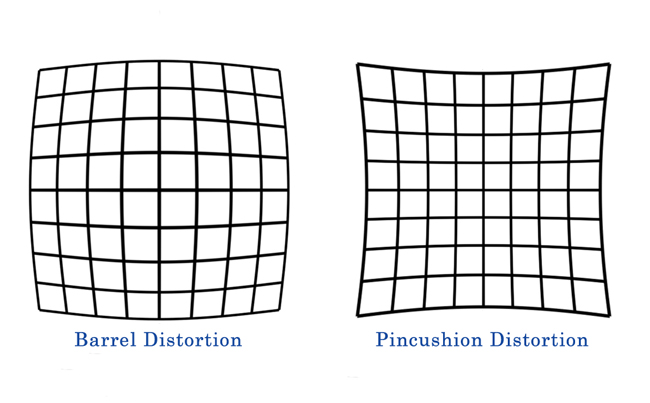
\includegraphics[width=240pt]{camera_distortion.jpg}
  \caption{左桶型畸变 右枕型畸变}
  \label{fig:radial_distort}
\end{figure}

切向畸变则是由于相机装配过程中,相机透镜平面与CMOS感光平面不完全平行造成
的,具体造成原因如图\ref{fig:tangential_distort}所示。尽管在各种相机校准
方法中,关于切向畸变 都有对应的处理手段,但是在实际工程应用中,由于切向
畸变一般较小,影响也 较小,因此大多数情况下都不予处理。THUR-20发布的标准
校准流程中,对切向 畸变也不予处理。

\begin{figure}[h] % use float package if you want it here
  \centering
  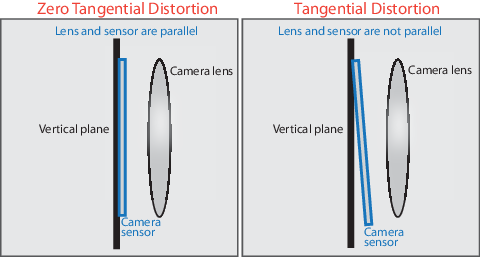
\includegraphics[width=300pt]{tangential_dist.png}
  \caption{左正常装配结果 右有装配误差的装配结果}
  \label{fig:tangential_distort}
\end{figure}

Kannala Brant模型使用光线的入射角$\theta$对图片上对应点的径向距离r进行拟合,
拟合形式如下式所示。

\begin{equation}
  r(\theta) = k_1\theta + k_2\theta^{3} + k_3\theta^{5} + k_4\theta^{7} + ...
\end{equation}

根据工程实践经验,THUR-20规范中,要求使用KB模型校准时,将$k_1$取为1,并对
拟合参数{k}取到5阶,即有效畸变参数为$[k_2, k_3, k_4, k_5]$。如图TODO为在
THUR-20数据采集过程中,使用KB模型校准后的顶视摄像头的RGB图片的修正前后
对比图。

为方便数据采集者开始工作,降低各位同行加入THUR-20数据采集工作的门槛,
笔者依赖OpenCV编写了相机内参标定程序,可兼容Kinect2、Kinect dk,realsense
并直接生成THUR-20需要的内参文件。辅助程序地址为:TODO


%\section{其它例子}
%\label{sec:other}

%在第~\ref{cha:intro} 章中我们学习了贝叶斯公式~(\ref{equ:chap1:bayes}),这里我们复
%习一下:
%\begin{equation}
%\label{equ:chap2:bayes}
%p(y|\vx) = \frac{p(\vx,y)}{p(\vx)}=
%\frac{p(\vx|y)p(y)}{p(\vx)}
%\end{equation}

%\subsection{绘图}
%\label{sec:draw}

%本模板不再预先装载任何绘图包(如 \pkg{pstricks,pgf} 等),完全由用户来决定。
%个人觉得 \pkg{pgf} 不错,不依赖于 Postscript。此外还有很多针对 \LaTeX{} 的
 %GUI 作图工具,如 XFig(jFig), WinFig, Tpx, Ipe, Dia, Inkscape, LaTeXPiX,
%jPicEdt, jaxdraw 等等。

%\subsection{插图}
%\label{sec:graphs}

%强烈推荐《\LaTeXe{} 插图指南》!关于子图形的使用细节请参看 \pkg{subcaption} 宏包的说明文档。

%\subsubsection{一个图形}
%\label{sec:onefig}
%一般图形都是处在浮动环境中。之所以称为浮动是指最终排版效果图形的位置不一定与源文
%件中的位置对应\footnote{This is not a bug, but a feature of \LaTeX!},这也是刚使
%用 \LaTeX{} 同学可能遇到的问题。如果要强制固定浮动图形的位置,请使用 \pkg{float} 宏包,
%它提供了 \texttt{[H]} 参数,比如图~\ref{fig:xfig1}。
%\begin{figure}[H] % use float package if you want it here
  %\centering
  %\includegraphics{thu-whole-logo.pdf}
  %\caption{利用 Xfig 制图}
  %\label{fig:xfig1}
%\end{figure}

%大学之道,在明明德,在亲民,在止于至善。知止而后有定;定而后能静;静而后能安;安
%而后能虑;虑而后能得。物有本末,事有终始。知所先后,则近道矣。古之欲明明德于天
%下者,先治其国;欲治其国者,先齐其家;欲齐其家者,先修其身;欲修其身者,先正其心;
%欲正其心者,先诚其意;欲诚其意者,先致其知;致知在格物。物格而后知至;知至而后
%意诚;意诚而后心正;心正而后身 修;身修而后家齐;家齐而后国治;国治而后天下
%平。自天子以至于庶人,壹是皆以修身为本。其本乱而未治者 否矣。其所厚者薄,而其所
%薄者厚,未之有也!

%\hfill —— 《大学》


%\subsubsection{多个图形}
%\label{sec:multifig}

%如果多个图形相互独立,并不共用一个图形计数器,那么
%用 \texttt{minipage} 或者\texttt{parbox} 就可以。否则,请参看
%图~\ref{fig:big1-subcaptionbox},它包含两个小图,分别是图~\ref{fig:subfig1}和
%图~\ref{fig:subfig2}。推荐使用 \cs{subcaptionbox},因为可以像
%图~\ref{fig:big1-subcaptionbox} 那样对齐子图的标题,也可以使用 \pkg{subcaption}
%宏包的 \cs{subcaption}(放在 minipage中,用法同\cs{caption})或
%是 \pkg{subfigure} 、\pkg{subtable}环境,像图~\ref{fig:big1-subfigure},不要再
%用 \cs{subfloat}、\cs{subfigure} 和 \cs{subtable}。

%\begin{figure}[h]
  %\centering%
  %\subcaptionbox{第一个小图形\label{fig:subfig1}}[3cm] %标题的长度,超过则会换行,如下一个小图。
    %{\includegraphics[height=3cm]{thu-fig-logo.pdf}}%
  %\hspace{4em}%
  %\subcaptionbox{第二个小图形,注意这个图略矮些。如果标题很长的话,它会自动换行\label{fig:subfig2}}
      %{\includegraphics[height=2cm]{thu-text-logo.pdf}}
  %\caption{包含子图形的大图形(subcaptionbox示例)}
  %\label{fig:big1-subcaptionbox}
%\end{figure}
%\begin{figure}[h]
  %\centering%
  %\begin{subfigure}{3cm}
    %\includegraphics[height=3cm]{thu-fig-logo.pdf}
    %\caption{第一个小图形}
  %\end{subfigure}%
  %\hspace{4em}%
  %\begin{subfigure}{0.5\textwidth}
    %\includegraphics[height=2cm]{thu-text-logo.pdf}
    %\caption{第二个小图形,注意这个图略矮些。subfigure中同一行的子图在顶端对齐。}
  %\end{subfigure}
  %\caption{包含子图形的大图形(subfigure示例)}
  %\label{fig:big1-subfigure}
%\end{figure}

%古之学者必有师。师者,所以传道受业解惑也。人非生而知之者,孰能无惑?惑而不从师,
%其为惑也,终不解矣。生乎吾前,其闻道也固先乎吾,吾从而师之;生乎吾後,其闻道也亦
%先乎吾,吾从而师之。吾师道也,夫庸知其年之先後生於吾乎!是故无贵无贱无长无少,道
%之所存,师之所存也。

%嗟乎!师道之不传也久矣,欲人之无惑也难矣。古之圣人,其出人也远矣,犹且从师而问焉;
%今之众人,其下圣人也亦远矣,而耻学於师。是故圣益圣,愚益愚。圣人之所以为圣,愚
%人之所以为愚,其皆出於此乎?爱其子,择师而教之,於其身也,则耻师焉,惑焉。彼童子
%之师,授之书而习其句读者,非吾所谓传其道、解其惑者也。句读之不知,惑之不解,或师
%焉,或不焉,小学而大遗,吾未见其明也。巫医、乐师、百工之人不耻相师,  士大夫之族
%曰“师”曰“弟子”之云者,则群聚而笑之。问之,则曰:彼与彼年相若也,道相似也,位
%卑则足羞,官盛则近谀。呜呼!师道之不复,可知矣。巫医、乐师、百工之人。吾子不齿,
%今其智乃反不能及,其可怪也欤!圣人无常师。孔子师郯子、苌子、师襄、老聃。郯子之徒,
%其贤不及孔子。孔子曰:“三人行,必有我师。”是故弟子不必不如师,师不必贤於弟子。
%闻道有先後,术业有专攻,如是而已。

%如果要把编号的两个图形并排,那么小页就非常有用了:
%\begin{figure}
%\begin{minipage}{0.48\textwidth}
  %\centering
  %\includegraphics[height=2cm]{thu-whole-logo.pdf}
  %\caption{并排第一个图}
  %\label{fig:parallel1}
%\end{minipage}\hfill
%\begin{minipage}{0.48\textwidth}
  %\centering
  %\includegraphics[height=2cm]{thu-whole-logo.pdf}
  %\caption{并排第二个图}
  %\label{fig:parallel2}
%\end{minipage}
%\end{figure}

%李氏子蟠,年十七,好古文、六艺,经传皆通习之,不拘於时,学於余。余嘉其能行古
%道,作师说以贻之。

%\hfill —— 韩愈(唐)
